%!TEX root = ../username.tex
\chapter{Realtime Audio Programming}
\hspace*{-0.12cm}This chapter will consider the theory behind audio programming and the different principles that are followed to create a functional program. It will begin with an overview of two types of signals: \textit{continuous signals} and \textit{discrete signals}. Next, it will cover the methods by which a digital system communicates with its speakers to create sound. After, the requirements that a realtime audio program needs in order to function will be considered. Specifically, this will include program structure and functionality. Finally, several libraries and other software available that handles these requirements will be discussed in length.
\section{Sound As A Discrete Signal}
Sound is a physical phenomenon. Vibrations travel though a medium such as air to create waves and differences in pressure, which travel at the the speed of sound (roughly 343 m/s). Naturally, representing this in a digital setting involves simplifying the physical nature of sound waves into an easily digestible format.

Consider Figure 3.1.

\begin{figure}[h] % [h] used to prevent {figure} from doing weird positioning
\begin{center}
	\fbox{
	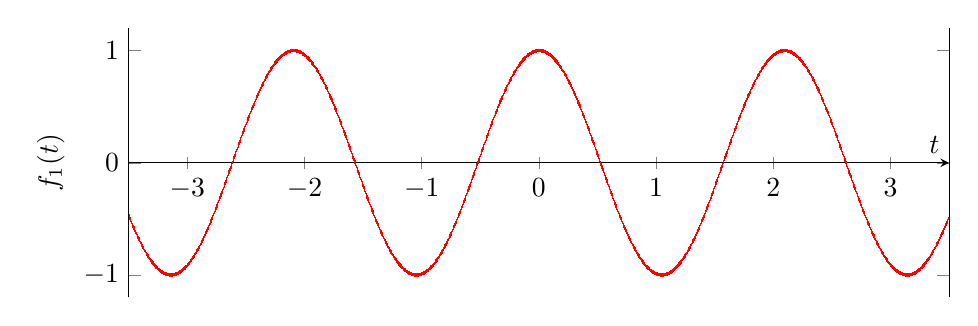
\begin{tikzpicture}
		\begin{axis} [
			axis x line = middle, % The x axis should go through the origin
			xlabel = \(t\),
			ylabel = {\(f_1(t)\)},
			height = 5cm,
			width = 12cm
			]

			\addplot [
			jump mark mid,
			domain = -3.5:3.5,
			samples = 1000,
			very thick, red
			] {(cos(deg(3 * x)))};

		\end{axis}
	\end{tikzpicture}}
	\caption{A graph of the sine wave \(f_1(t) = cos(3t)\).}
\end{center}
\end{figure}

This is a representation of a sinusoid under the time domain. Each crest and trough represent the difference in air pressure that occurs when this tone is created. By graphing the sinusoid with respect to time, one can view the particular waveform that is created from this given sound. This representation describes one particular type of signal: \textit{continuous sinusoidal signals}. These are defined by the following expression:

\begin{defn}[Definition of a continuous sinusoid]\label{def1}
	\begin{equation}\label{introf(t)}
	f(t)=Acos(2\pi ft + \varTheta), t \in (-\infty, \infty)
\end{equation}\end{defn}

where \textit{f} is frequency, \textit{t} is time, and $\varTheta$ is the phase offset in radians \cite{Symons_2013}. One is not limited to sinusoids, however. One can create (or deconstruct) any type of non-sinusoidal signal by taking the sum of several sinusoids to approximate a desired signal, given a sufficiently high number of sine waves are used. This is defined as:

\begin{defn}[Definition of a non-sinusoidal continuous signal]\label{def1}
	\begin{equation}\label{intro2f(t)}
	f(t)=\sum_{k=1}^{N_h} A_k cos(2\pi kft + \varTheta_k)
\end{equation}\end{defn}

where \textit{k} is one sinusoid in the sum, $N_h$ is the number of total sinusoids used to construct the signal, $A_k$ the amplitude of a particular signal for each \textit{k}, $\varTheta_k$ the phase for each \textit{k}, and \textit{f} the fundamental frequency of $f(t)$ \cite{Symons_2013}.

One can represent Figure 3.1 digitally by taking measurements of the function \(f_1(t)\) at regular points in time, each known as a \textit{sample}. By convention, samples are in the range (-1,1). By graphing each sample into the function \(f_2(t)\), one can create a digital version of this analog signal.

\begin{figure}[h] % [h] used to prevent {figure} from doing weird positioning
	\begin{center}
		\fbox{
		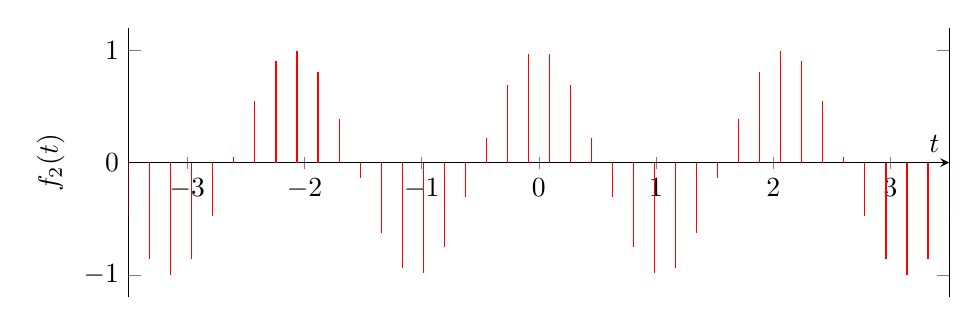
\begin{tikzpicture}
			\begin{axis} [
				axis x line = middle, % The x axis should go through the origin
				xlabel = \(t\),
				ylabel = {\(f_2(t)\)},
				height = 5cm,
				width = 12cm
				]

				\addplot+ [
				ycomb,
				mark = text,
				text mark = , % so jank
				domain = -3.5:3.5,
				samples = 40,
				red
				] {(cos(deg(3 * x)))};

			\end{axis}
		\end{tikzpicture}
		}
		\caption{A discrete graph of the sine wave \(f_2(t) = cos(3t)\) taken with 40 samples.}
	\end{center}
\end{figure}

This is a discrete representation of our original graph \(f_1(t) = sin(3t)\). []



\section{The Realtime Programming Bus Schedule}
[] Unlike a music player, our program has to follow the set schedule requested by the audio driver of a device [].
\section{The Golden Rules}
\section{Software Available}
